\documentclass{ximera}

 

\usepackage{epsfig}

\graphicspath{
  {./}
  {figures/}
}

\usepackage{morewrites}
\makeatletter
\newcommand\subfile[1]{%
\renewcommand{\input}[1]{}%
\begingroup\skip@preamble\otherinput{#1}\endgroup\par\vspace{\topsep}
\let\input\otherinput}
\makeatother

\newcommand{\includeexercises}{\directlua{dofile("/home/jim/linearAlgebra/laode/exercises.lua")}}

%\newcounter{ccounter}
%\setcounter{ccounter}{1}
%\newcommand{\Chapter}[1]{\setcounter{chapter}{\arabic{ccounter}}\chapter{#1}\addtocounter{ccounter}{1}}

%\newcommand{\section}[1]{\section{#1}\setcounter{thm}{0}\setcounter{equation}{0}}

%\renewcommand{\theequation}{\arabic{chapter}.\arabic{section}.\arabic{equation}}
%\renewcommand{\thefigure}{\arabic{chapter}.\arabic{figure}}
%\renewcommand{\thetable}{\arabic{chapter}.\arabic{table}}

%\newcommand{\Sec}[2]{\section{#1}\markright{\arabic{ccounter}.\arabic{section}.#2}\setcounter{equation}{0}\setcounter{thm}{0}\setcounter{figure}{0}}

\newcommand{\Sec}[2]{\section{#1}}

\setcounter{secnumdepth}{2}
%\setcounter{secnumdepth}{1} 

%\newcounter{THM}
%\renewcommand{\theTHM}{\arabic{chapter}.\arabic{section}}

\newcommand{\trademark}{{R\!\!\!\!\!\bigcirc}}
%\newtheorem{exercise}{}

\newcommand{\dfield}{{\sf dfield9}}
\newcommand{\pplane}{{\sf pplane9}}

\newcommand{\EXER}{\section*{Exercises}}%\vspace*{0.2in}\hrule\small\setcounter{exercise}{0}}
\newcommand{\CEXER}{}%\vspace{0.08in}\begin{center}Computer Exercises\end{center}}
\newcommand{\TEXER}{} %\vspace{0.08in}\begin{center}Hand Exercises\end{center}}
\newcommand{\AEXER}{} %\vspace{0.08in}\begin{center}Hand Exercises\end{center}}

% BADBAD: \newcommand{\Bbb}{\bf}

\newcommand{\R}{\mbox{$\Bbb{R}$}}
\newcommand{\C}{\mbox{$\Bbb{C}$}}
\newcommand{\Z}{\mbox{$\Bbb{Z}$}}
\newcommand{\N}{\mbox{$\Bbb{N}$}}
\newcommand{\D}{\mbox{{\bf D}}}
\usepackage{amssymb}
%\newcommand{\qed}{\hfill\mbox{\raggedright$\square$} \vspace{1ex}}
%\newcommand{\proof}{\noindent {\bf Proof:} \hspace{0.1in}}

\newcommand{\setmin}{\;\mbox{--}\;}
\newcommand{\Matlab}{{M\small{AT\-LAB}} }
\newcommand{\Matlabp}{{M\small{AT\-LAB}}}
\newcommand{\computer}{\Matlab Instructions}
\newcommand{\half}{\mbox{$\frac{1}{2}$}}
\newcommand{\compose}{\raisebox{.15ex}{\mbox{{\scriptsize$\circ$}}}}
\newcommand{\AND}{\quad\mbox{and}\quad}
\newcommand{\vect}[2]{\left(\begin{array}{c} #1_1 \\ \vdots \\
 #1_{#2}\end{array}\right)}
\newcommand{\mattwo}[4]{\left(\begin{array}{rr} #1 & #2\\ #3
&#4\end{array}\right)}
\newcommand{\mattwoc}[4]{\left(\begin{array}{cc} #1 & #2\\ #3
&#4\end{array}\right)}
\newcommand{\vectwo}[2]{\left(\begin{array}{r} #1 \\ #2\end{array}\right)}
\newcommand{\vectwoc}[2]{\left(\begin{array}{c} #1 \\ #2\end{array}\right)}

\newcommand{\ignore}[1]{}


\newcommand{\inv}{^{-1}}
\newcommand{\CC}{{\cal C}}
\newcommand{\CCone}{\CC^1}
\newcommand{\Span}{{\rm span}}
\newcommand{\rank}{{\rm rank}}
\newcommand{\trace}{{\rm tr}}
\newcommand{\RE}{{\rm Re}}
\newcommand{\IM}{{\rm Im}}
\newcommand{\nulls}{{\rm null\;space}}

\newcommand{\dps}{\displaystyle}
\newcommand{\arraystart}{\renewcommand{\arraystretch}{1.8}}
\newcommand{\arrayfinish}{\renewcommand{\arraystretch}{1.2}}
\newcommand{\Start}[1]{\vspace{0.08in}\noindent {\bf Section~\ref{#1}}}
\newcommand{\exer}[1]{\noindent {\bf \ref{#1}}}
\newcommand{\ans}{}
\newcommand{\matthree}[9]{\left(\begin{array}{rrr} #1 & #2 & #3 \\ #4 & #5 & #6
\\ #7 & #8 & #9\end{array}\right)}
\newcommand{\cvectwo}[2]{\left(\begin{array}{c} #1 \\ #2\end{array}\right)}
\newcommand{\cmatthree}[9]{\left(\begin{array}{ccc} #1 & #2 & #3 \\ #4 & #5 &
#6 \\ #7 & #8 & #9\end{array}\right)}
\newcommand{\vecthree}[3]{\left(\begin{array}{r} #1 \\ #2 \\
#3\end{array}\right)}
\newcommand{\cvecthree}[3]{\left(\begin{array}{c} #1 \\ #2 \\
#3\end{array}\right)}
\newcommand{\cmattwo}[4]{\left(\begin{array}{cc} #1 & #2\\ #3
&#4\end{array}\right)}

\newcommand{\Matrix}[1]{\ensuremath{\left(\begin{array}{rrrrrrrrrrrrrrrrrr} #1 \end{array}\right)}}

\newcommand{\Matrixc}[1]{\ensuremath{\left(\begin{array}{cccccccccccc} #1 \end{array}\right)}}



\renewcommand{\labelenumi}{\theenumi)}
\newenvironment{enumeratea}%
{\begingroup
 \renewcommand{\theenumi}{\alph{enumi}}
 \renewcommand{\labelenumi}{(\theenumi)}
 \begin{enumerate}}
 {\end{enumerate}\endgroup}



\newcounter{help}
\renewcommand{\thehelp}{\thesection.\arabic{equation}}

%\newenvironment{equation*}%
%{\renewcommand\endequation{\eqno (\theequation)* $$}%
%   \begin{equation}}%
%   {\end{equation}\renewcommand\endequation{\eqno \@eqnnum
%$$\global\@ignoretrue}}

%\input{psfig.tex}

\author{Martin Golubitsky and Michael Dellnitz}

%\newenvironment{matlabEquation}%
%{\renewcommand\endequation{\eqno (\theequation*) $$}%
%   \begin{equation}}%
%   {\end{equation}\renewcommand\endequation{\eqno \@eqnnum
% $$\global\@ignoretrue}}

\newcommand{\soln}{\textbf{Solution:} }
\newcommand{\exercap}[1]{\centerline{Figure~\ref{#1}}}
\newcommand{\exercaptwo}[1]{\centerline{Figure~\ref{#1}a\hspace{2.1in}
Figure~\ref{#1}b}}
\newcommand{\exercapthree}[1]{\centerline{Figure~\ref{#1}a\hspace{1.2in}
Figure~\ref{#1}b\hspace{1.2in}Figure~\ref{#1}c}}
\newcommand{\para}{\hspace{0.4in}}

\renewenvironment{solution}{\suppress}{\endsuppress}

\ifxake
\newenvironment{matlabEquation}{\begin{equation}}{\end{equation}}
\else
\newenvironment{matlabEquation}%
{\let\oldtheequation\theequation\renewcommand{\theequation}{\oldtheequation*}\begin{equation}}%
  {\end{equation}\let\theequation\oldtheequation}
\fi

\makeatother


\title{Vectors and Matrices in Coordinates}

\begin{document}
\begin{abstract}
\end{abstract}
\maketitle

  \label{S:coordinates}

In the last half of this chapter we discuss how similarity of matrices should
be thought of as change of coordinates for linear mappings.  There are three
steps in this discussion.
\begin{enumerate}
\item 	Formalize the idea of coordinates for a vector in terms of basis.
\item	Discuss how to write a linear map as a matrix in each coordinate
	system.
\item	Determine how the matrices corresponding to the same linear map in
	two different coordinate systems are related.
 \end{enumerate}
The answer to the last question is simple: the matrices are related by a
change of coordinates if and only if they are similar.  We discuss these
steps in this section in $\R^n$ and in Section~\ref{MALT} for general vector
spaces.


\subsection*{Coordinates of Vectors using Bases}

Throughout, we have written vectors $v\in\R^n$ in coordinates as
$v = (v_1,\ldots,v_n)$, and we have used this notation almost without
comment.  From the point of view of vector space operations, we are
just writing
\[
v = v_1e_1 + \cdots + v_ne_n
\]
as a linear combination \index{linear!combination} of the standard basis
${\cal E} = \{e_1,\ldots,e_n\}$ of $\R^n$.

More generally, each basis provides a set of coordinates for a vector space.
This fact is described by the following lemma (although its proof is identical 
to the first part of the proof of Theorem~\ref{L:linmapfrombasis} in 
Chapter~\ref{C:vectorspaces}).

\begin{lemma} \label{L:coordinates}
Let ${\cal W}=\{w_1,\ldots,w_n\}$ be a basis for the vector space $V$.  Then
each vector $v$ in $V$ can be written uniquely as a linear combination of
vectors in ${\cal W}$; that is,
\[
v = \alpha_1w_1 +\cdots + \alpha_nw_n,
\]
for uniquely defined scalars $\alpha_1,\ldots,\alpha_n$.
\end{lemma}

\begin{proof}  Since ${\cal W}$ is a basis, Theorem~\ref{basis=span+indep} of
Chapter~\ref{C:vectorspaces} implies that the vectors $w_1,\ldots,w_n$ span
$V$ and are linearly independent.  Therefore, we can write $v$ in $V$ as a
linear combination of vectors in ${\cal B}$.   That is, there are scalars
$\alpha_1,\ldots,\alpha_n$ such that
\[
v = \alpha_1w_1 +\cdots + \alpha_nw_n.
\]
Next we show that these scalars are uniquely defined.  Suppose that we can 
write $v$ as a linear combination of the vectors in ${\cal B}$ in a second 
way; that is, suppose 
\[
v = \beta_1w_1 + \cdots + \beta_nw_n
\]
for scalars $\beta_1,\ldots,\beta_n$.  Then
\[
(\alpha_1-\beta_1)w_1 + \cdots + (\alpha_n-\beta_n)w_n = 0.
\]
Since the vectors in ${\cal W}$ are linearly independent, it
follows that $\alpha_j=\beta_j$ for all $j$.  \end{proof}

\begin{Def}  \label{D:coordinates}
Let ${\cal W} = \{w_1,\ldots,w_n\}$ be a basis in a vector space $V$.
Lemma~\ref{L:coordinates} states that we can write $v\in V$ uniquely as
\begin{equation}  \label{e:coordv}
v = \alpha_1w_1 + \cdots + \alpha_nw_n.
\end{equation}
The scalars $\alpha_1,\ldots,\alpha_n$ are the {\em coordinates\/} of $v$
relative to the basis ${\cal W}$, and we denote the coordinates of $v$ in
the basis ${\cal W}$ by
\begin{equation}   \label{e:coordnot}
[v]_{\cal W} = (\alpha_1,\ldots,\alpha_n) \in\R^n.
\end{equation}
\end{Def}\index{coordinates}\index{vector!coordinates}

We call the coordinates of a vector $v\in\R^n$ relative to the standard basis,
the {\em standard coordinates\/}\index{coordinates!standard} of $v$.

\subsection*{Writing Linear Maps in Coordinates as Matrices}

Let $V$ be a finite dimensional vector space of dimension\index{dimension}
$n$ and let
$L:V\to V$ be a linear mapping\index{linear!mapping}.
We now show how each basis of $V$ allows
us to associate an $n\times n$ matrix to $L$.  Previously we considered
this question with the standard basis on $V=\R^n$. We showed in
Chapter~\ref{chap:matrices} that
we can write the linear mapping $L$ as a
matrix mapping\index{matrix!mappings}, as
follows.  Let ${\cal E}=\{e_1,\ldots,e_n\}$ be the standard
basis in $\R^n$.  Let $A$ be the $n\times n$ matrix whose
$j^{th}$ column is the $n$ vector $L(e_j)$.  Then
Chapter~\ref{chap:matrices}, Theorem~\ref{lin-matrices} shows
that the linear map is given by matrix multiplication as
\[
L(v) = Av.
\]
Thus every linear mapping on $\R^n$ can be written in this matrix form.

\begin{rmk} \label{R:standard} {\rm
Another way to think of the $j^{th}$ column of the matrix $A$
is as the coordinate vector of $L(e_j)$ relative to the
standard basis, that is, as $[L(e_j)]_{\cal E}$.  We denote the
matrix $A$ by $[L]_{\cal E}$; this notation emphasizes the fact
that $A$ is the matrix of $L$ relative to the standard basis.}
\end{rmk}


We now discuss how to write a linear map $L$ as a matrix using
different coordinates.
\begin{Def} \label{D:matrixincoord}
Let ${\cal W} = \{w_1,\ldots,w_n\}$ be a basis for the vector
space $V$. The $n\times n$ matrix $[L]_{\cal W}$ associated to
the linear map $L:V\to V$ and the basis ${\cal W}$ is defined
as follows.  The $j^{th}$ column of $[L]_{\cal W}$ is
$[L(w_j)]_{\cal W}$ --- the coordinates of $L(w_j)$ relative
to the basis ${\cal W}$.
\end{Def} \index{matrix!associated to a linear map}

Note that when $V=\R^n$ and when ${\cal W} = {\cal E}$, the
standard basis of $\R^n$, then the definition of the matrix
$[L]_{\cal E}$ is exactly the same as the matrix associated
with the linear map $L$ in Remark~\ref{R:standard}.

\begin{lemma}
The coordinate vector of $L(v)$ relative to the basis ${\cal W}$ is
\begin{equation} \label{e:matrixofL}
[L(v)]_{\cal W} = [L]_{\cal W} [v]_{\cal W}.
\end{equation}
\end{lemma}  \index{coordinates}

\begin{proof} The process of choosing the coordinates of vectors relative to
a given basis ${\cal W} =\{w_1,\ldots,w_n\}$ of a vector space $V$
is itself linear.  Indeed,
\begin{eqnarray*}
[u+v]_{\cal W} & = & [u]_{\cal W} + [v]_{\cal W} \\
  \; [cv]_{\cal W}  & = &  c[v]_{\cal W}.
\end{eqnarray*}
Thus the coordinate mapping relative to a basis ${\cal W}$ of $V$
defined by
\begin{equation}  \label{e:coordmap}
v \mapsto [v]_{\cal W}
\end{equation}
is a linear mapping of $V$ into $\R^n$.  We denote this linear
mapping by $[\cdot]_{\cal W}:V\to\R^n$.


It now follows that both the left hand and right hand sides of
\Ref{e:matrixofL} can be thought of as linear mappings of $V\to\R^n$.
In verifying this comment, we recall Lemma~\ref{L:compose} of
Chapter~\ref{C:vectorspaces} that states that the composition of linear
maps is linear.  On the left hand side we have the mapping
\[
v \mapsto L(v) \mapsto [L(v)]_{\cal W},
\]
which is the composition of the linear maps: $[\cdot]_{\cal W}$ with
$L$.  See \Ref{e:coordmap}.  The right hand side is
\[
v \mapsto [v]_{\cal W} \mapsto [L]_{\cal W} [v]_{\cal W},
\]
which is the composition of the linear maps:  multiplication by the
matrix $[L]_{\cal W}$ with $[\cdot]_{\cal W}$.

Theorem~\ref{L:linmapfrombasis} of Chapter~\ref{C:vectorspaces}
states that linear mappings are determined by their actions on a
basis.  Thus to verify \Ref{e:matrixofL}, we need only verify this
equality for $v=w_j$ for all $j$.  Since $[w_j]_{\cal W}=e_j$, the right
hand side of \Ref{e:matrixofL} is:
\[
[L]_{\cal W} [w_j]_{\cal W} =  [L]_{\cal W} e_j,
\]
which is just the $j^{th}$ column of $[L]_{\cal W}$.  The left hand side of
\Ref{e:matrixofL} is the vector $[L(w_j)]_{\cal W}$, which by definition is
also the $j^{th}$ column of $[L]_{\cal W}$
(see Definition~\ref{D:matrixincoord}).    \end{proof}


\subsection*{Computations of Vectors in Coordinates in $\R^n$}
\index{coordinates}

We divide this subsection into three parts.  We consider a simple example in
$\R^2$ algebraically in the first part and geometrically in the second.  In
the third part we formalize and extend the algebraic discussion to $\R^n$.

\subsubsection*{An Example of Coordinates in $\R^2$}
\index{coordinates!in ${\bf R}^2$}

How do we find the coordinates of a vector $v$ in a basis?  For example,
choose a (nonstandard) basis in the plane --- say
\[
w_1=(1,1) \AND w_2=(1,-2).
\]
Since $\{w_1,w_2\}$ is a basis, we may write the vector
$v$ as a linear combination of the vectors $w_1$ and
$w_2$.  Thus we can find scalars $\alpha_1$ and $\alpha_2$ so
that
\[
v=\alpha_1 w_1 + \alpha_2 w_2 = \alpha_1(1,1)+\alpha_2(1,-2)
= (\alpha_1+ \alpha_2,\alpha_1 -2 \alpha_2).
\]
In standard coordinates, set $v=(v_1,v_2)$; this equation leads to the
system of linear equations
\begin{eqnarray*}
v_1 & = & \alpha_1 + \alpha_2 \\
v_2 & = & \alpha_1 -2 \alpha_2
\end{eqnarray*}
in the two variables $\alpha_1$ and $\alpha_2$. As we have seen,
the fact that $w_1$ and $w_2$ form a basis of $\R^2$ implies that
these equations do have a solution.  Indeed, we can write this
system in matrix form as
\[
\vectwo{v_1}{v_2} = \mattwo{1}{1}{1}{-2}\vectwo{\alpha_1}{\alpha_2},
\]
which is solved by inverting the matrix to obtain:
\begin{equation} \label{change1}
\vectwo{\alpha_1}{\alpha_2}= \frac{1}{3}\mattwo{2}{1}{1}{-1}
\vectwo{v_1}{v_2}.
\end{equation}
For example, suppose $v=(2.0,0.5)$.  Using \Ref{change1} we find that
$(\alpha_1,\alpha_2)=(1.5,0.5)$; that is, we can write
\[
v = 1.5w_1 + 0.5w_2,
\]
and $(1.5,0.5)$ are the {\em coordinates\/} \index{coordinates} of
$v$ in the basis $\{w_1,w_2\}$.

Using the notation in \Ref{e:coordnot}, we may rewrite \Ref{change1} as
\[
[v]_{\cal W} = \frac{1}{3}\mattwo{2}{1}{1}{-1} [v]_{\cal E},
\]
where ${\cal E} = \{e_1,e_2\}$ is the standard basis.

\subsubsection*{Planar Coordinates Viewed Geometrically using \Matlab}
\index{coordinates!in \Matlab}

Next we use \Matlab to view geometrically the notion of coordinates
relative to a basis ${\cal W}=\{w_1,w_2\}$ in the plane.  Type
\begin{verbatim}
w1 = [1 1];
w2 = [1 -2];
bcoord
\end{verbatim} \index{\computer!bcoord}
\Matlab will create a graphics window showing the two basis vectors
$w_1$ and $w_2$ in red.  Using the mouse click on a point near
$(2,0.5)$ in that figure.  \Matlab will respond by plotting the
new vector $v$ in yellow and the parallelogram generated by
$\alpha_1w_1$ and $\alpha_2w_2$ in cyan.  The values of $\alpha_1$
and $\alpha_2$ are also plotted on this figure.  See
Figure~\ref{F:coords}.

\begin{figure}[htb]
     \centerline{%
     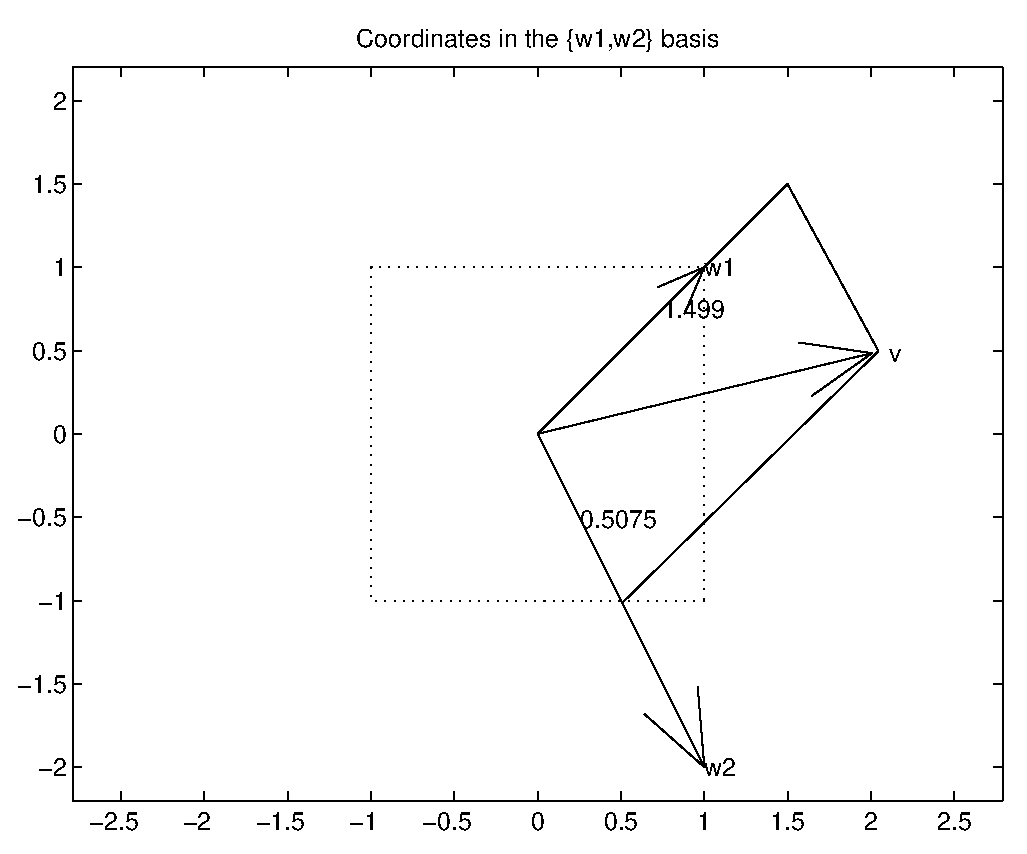
\psfig{file=../figures/coord.eps,width=3.5in}}
     \caption{The coordinates of $v=(2.0,0.5)$ in the basis
	$w_1=(1,1), w_2=(1,-2)$.}
     \label{F:coords}
\end{figure}

\subsubsection*{Abstracting $\R^2$ to $\R^n$}
\index{coordinates!in ${\bf R}^n$}

Suppose that we are given a basis ${\cal W} = \{w_1,\ldots,w_n\}$ of
$\R^n$ and a vector $v\in\R^n$.  How do we find the coordinates
$[v]_{\cal W}$ of $v$ in the basis ${\cal W}$?

For definiteness, assume that $v$ and the $w_j$ are row vectors.  Equation
\Ref{e:coordv} may be rewritten as
\[
v^t = (w_1^t|\cdots|w_n^t)\vect{\alpha}{n}.
\]
Thus,
\begin{equation}  \label{e:coordRn}
[v]_{\cal W} = \vect{\alpha}{n} = P_{\cal W}\inv v^t,
\end{equation}
where $P_{\cal W} = (w_1^t|\cdots|w_n^t)$.  Since the $w_j$ are a basis for
$\R^n$, the columns of the matrix $P_{\cal W}$ are linearly independent, and
$P_{\cal W}$ is invertible.


We may use \Ref{e:coordRn} to compute $[v]_{\cal W}$ using
\Matlabp.  For example, let
\[
v  =  (4,1,3)
\]
and
\[
w_1 =  (1,4,7) \quad w_2 = (2,1,0) \quad w_3 = (-4,2,1).
\]
Then $[v]_{\cal W}$ is found by typing
\begin{verbatim}
w1 = [ 1 4 7];
w2 = [ 2 1 0];
w3 = [-4 2 1];
inv([w1' w2' w3'])*[4 1 3]'
\end{verbatim} \index{\computer!inv}  \index{\computer!'}
The answer is:

\begin{verbatim}
ans =
    0.5306
    0.3061
   -0.7143
\end{verbatim}


\subsection*{Determining the Matrix of a Linear Mapping in Coordinates}

Suppose that we are given the linear map $L_A:\R^n\to\R^n$ associated to
the matrix $A$ in standard coordinates and a basis $w_1,\ldots,w_n$ of $\R^n$.
How do we find the matrix $[L_A]_{\cal W}$. As above, we assume that the
vectors $w_j$ and the vector $v$ are row vectors  Since $L_A(v)=Av^t$ we can
rewrite \Ref{e:matrixofL} as
\[
[L_A]_{\cal W}[v]_{\cal W} = [Av^t]_{\cal W}
\]
As above, let $P_{\cal W}=(w_1^t|\cdots|w_n^t)$.  Using \Ref{e:coordRn} we
see that
\[
[L_A]_{\cal W}P_{\cal W}\inv v^t = P_{\cal W}\inv Av^t.
\]
Setting
\[
u= P_{\cal W}\inv v^t
\]
we see that
\[
[L_A]_{\cal W}u = P_{\cal W}\inv A P_{\cal W}u.
\]
Therefore,
\[
[L_A]_{\cal W} = P_{\cal W}\inv AP_{\cal W}.
\]
We have proved:
\begin{thm}
Let $A$ be an $n\times n$ matrix and let $L_A:\R^n\to\R^n$ be the associated
linear map.  Let ${\cal W} = \{w_1,\ldots,w_n\}$ be a basis\index{basis} for
$\R^n$.  Then the matrix $[L_A]_{\cal W}$ associated to to $L_A$ in the basis
${\cal W}$ is similar\index{similar} to $A$.  Therefore the determinant, trace,
and eigenvalues of $[L_A]_{\cal W}$ are identical to those of $A$.
\end{thm}




\subsection*{Matrix Normal Forms in $\R^2$} \index{normal form}

If we are careful about how we choose the basis ${\cal W}$, then
we can simplify the form of the matrix $[L]_{\cal W}$.  Indeed, we
have already seen examples of this process when we discussed how
to find closed form solutions to linear planar systems of ODEs in
the previous chapter.  For example, suppose that $L:\R^2\to\R^2$
has real eigenvalues $\lambda_1$ and $\lambda_2$ with two
linearly independent eigenvectors $w_1$ and $w_2$.  Then the
matrix associated to $L$ in the basis ${\cal W} = \{w_1,w_2\}$
is the diagonal matrix
\begin{equation}   \label{e:diagcoord}
[L]_{\cal W} = \mattwo{\lambda_1}{0}{0}{\lambda_2},
\end{equation}
since
\[
[L(w_1)]_{\cal W} = [\lambda_1w_1]_{\cal W} = \vectwo{\lambda_1}{0} \AND
[L(w_2)]_{\cal W} = [\lambda_2w_2]_{\cal W} = \vectwo{0}{\lambda_2}.
\]

In Chapter~\ref{Chap:Planar} we showed how to classify $2\times 2$
matrices up to similarity (see Chapter~\ref{Chap:Planar},
Theorem~\ref{T:putinform}) and how to use this classification to find
closed form solutions to planar systems of linear ODEs (see
Section~\ref{S:6.5}).  We now use
the ideas of coordinates and matrices associated with bases to
reinterpret the normal form result (Chapter~\ref{Chap:Planar},
Theorem~\ref{T:putinform}) in a more geometric fashion.

\begin{thm}  \label{T:putinform2}
Let $L:\R^2\to\R^2$ be a linear mapping.  Then in an appropriate
coordinate system defined by the basis ${\cal W}$ below, the matrix
$L_{\cal W}$ has one of the following forms.
\begin{itemize}
\item[(a)]	Suppose that $L$ has two linearly independent
real eigenvectors $w_1$ and $w_2$ with real eigenvalues $\lambda_1$
and $\lambda_2$.  Then
\[
[L]_{\cal W} = \mattwo{\lambda_1}{0}{0}{\lambda_2}.
\]

\item[(b)]	Suppose that $L$ has no real eigenvectors and
complex conjugate eigenvalues $\sigma\pm i\tau$ where
$\tau\neq 0$.  Let $w_1+iw_2$ be a complex eigenvector of $L$
associated with the eigenvalue $\sigma-i\tau$.
Then ${\cal W}=\{w_1,w_2\}$ is a basis and
\[
[L]_{\cal W} = \mattwo{\sigma}{-\tau}{\tau}{\sigma}.
\]

\item[(c)]	Suppose that $L$ has exactly one linearly
independent real eigenvector $w_1$ with real eigenvalue $\lambda$.
Choose the generalized eigenvector\index{eigenvector!generalized} $w_2$
\begin{equation}  \label{e:Lw=lw+v}
(L-\lambda I_2)(w_2) =  w_1.
\end{equation}
Then ${\cal W}=\{w_1,w_2\}$ is a basis and
\[
[L]_{\cal W} = \mattwo{\lambda}{1}{0}{\lambda}.
\]
\end{itemize}
\end{thm}

\begin{proof}
The verification of (a) was discussed in \Ref{e:diagcoord}.  The
verification of (b) follows from Chapter~\ref{Chap:Planar},
\Ref{e:complexcoord} on equating $w_1$ with $v$ and $w_2$ with $w$.
The verification of (c) follows directly from \Ref{e:Lw=lw+v} as
\[
[L(w_1)]_{\cal W} = \lambda e_1 \AND [L(w_2)]_{\cal W} = e_1+\lambda e_2.
\]
\end{proof}



\subsubsection*{Visualization of Coordinate Changes in ODEs}
\index{change of coordinates}

We consider two examples.  As a first example note that the matrices
\[
C = \mattwo{1}{0}{0}{-2} \AND B = \mattwo{4}{-3}{6}{-5},
\]
are similar matrices.   Indeed, $B = P\inv CP$ where
\begin{equation}  \label{e:Pchange}
P = \mattwo{2}{-1}{1}{-1}.
\end{equation}
The phase portraits of the differential equations $\dot{X}=BX$ and
$\dot{X}=CX$ are shown in Figure~\ref{F:comparesim}.  Note that both
phase portraits are pictures of the {\em same\/} saddle\index{saddle} ---
just in different coordinate systems\index{coordinate system}.

\begin{figure}[htb]
        \centerline{%
        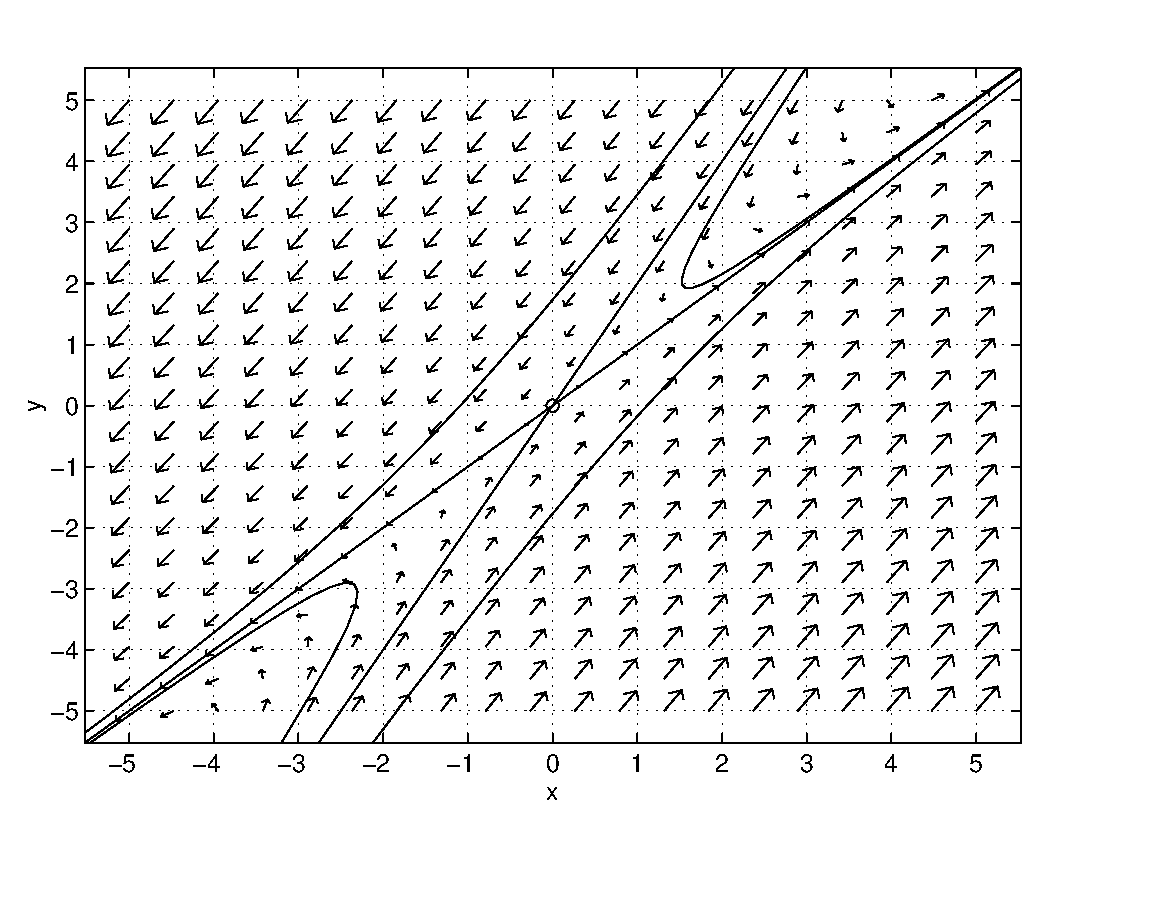
\psfig{file=../figures/saddle7a.eps,width=3.2in}
        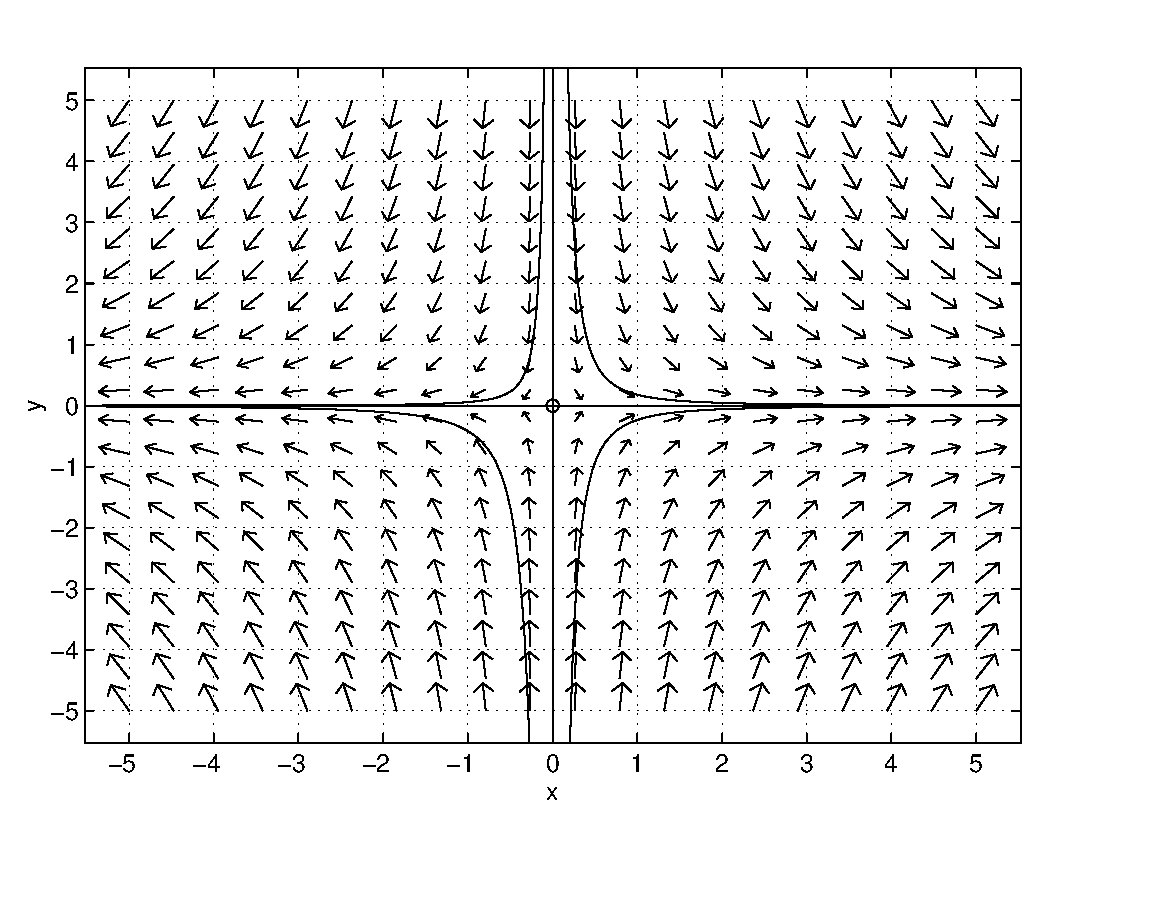
\psfig{file=../figures/saddle7b.eps,width=3.2in}}
        \caption{Phase planes for the saddles $\dot{X}=BX$ and $\dot{X}=CX$.}
        \label{F:comparesim}
\end{figure}

As a second example note that the matrices
\[
C = \mattwo{0}{2}{-2}{0} \AND B = \mattwo{6}{-4}{10}{-6}
\]
are similar matrices, and both are centers.   Indeed, $B = P\inv CP$
where $P$ is the same matrix as in \Ref{e:Pchange}.  The phase portraits
of the differential equations $\dot{X}=BX$ and $\dot{X}=CX$ are shown in
Figure~\ref{F:comparesim2}.  Note that both phase portraits are pictures
of the {\em same\/} center\index{center} --- just in different coordinate
systems.



\begin{figure}[htb]
        \centerline{%
        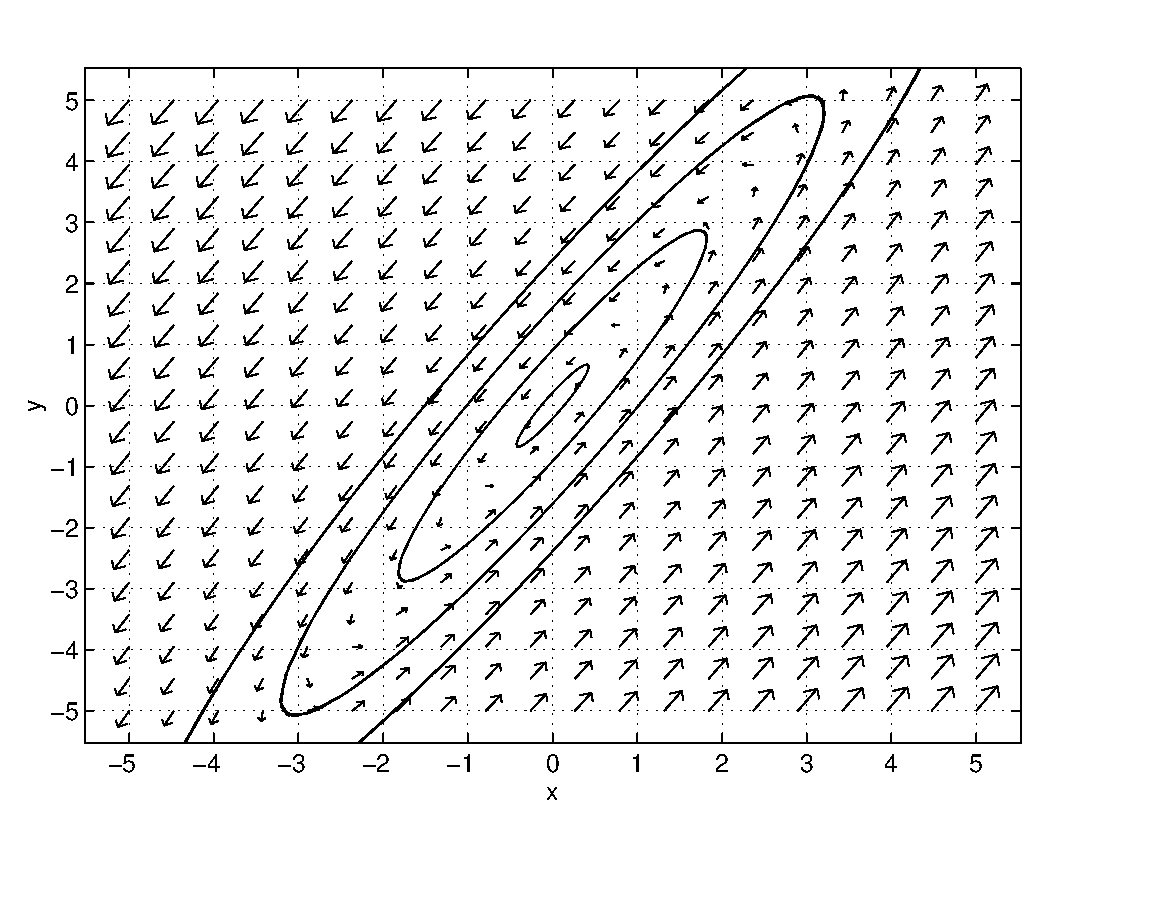
\psfig{file=../figures/center7a.eps,width=3.2in}
        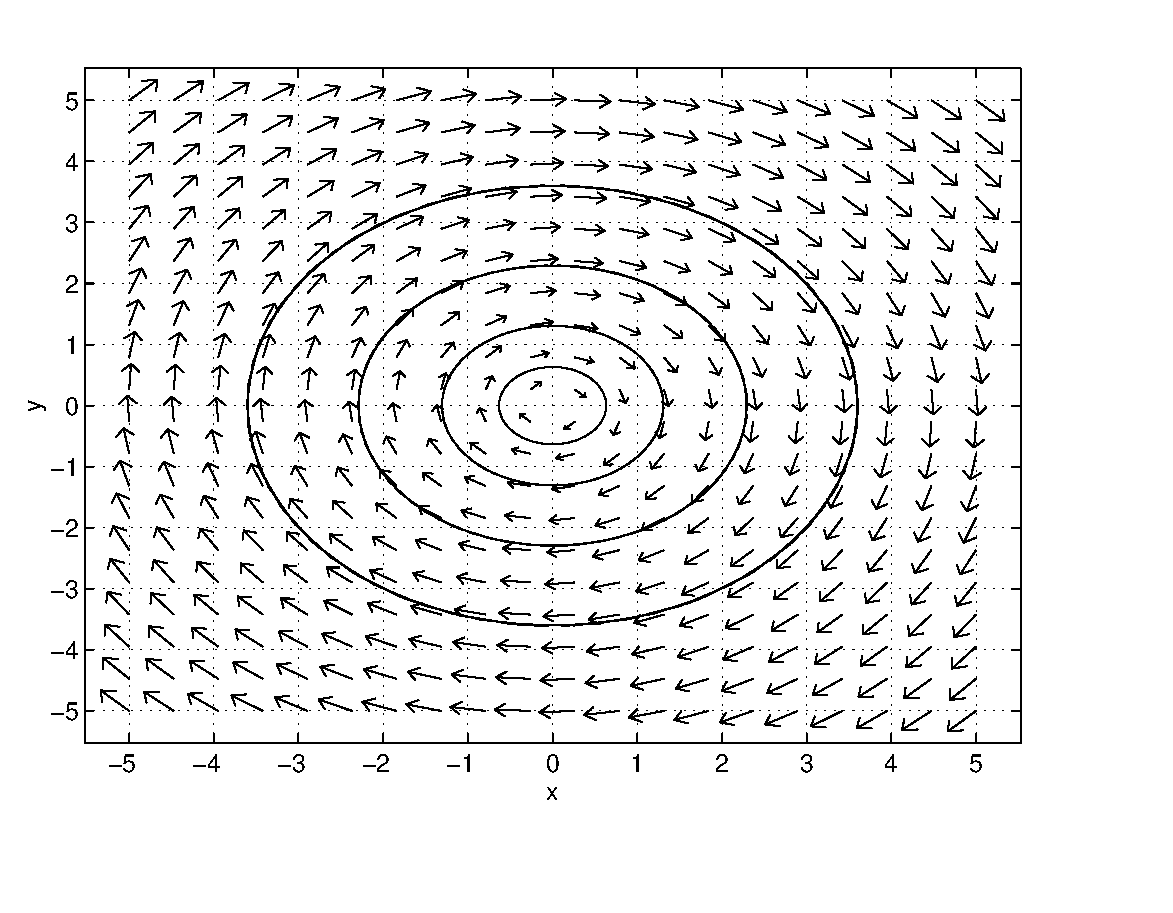
\psfig{file=../figures/center7b.eps,width=3.2in}}
        \caption{Phase planes for the centers $\dot{X}=BX$ and $\dot{X}=CX$.}
        \label{F:comparesim2}
\end{figure}






\EXER

\TEXER

\begin{exercise} \label{c7.1.1}
Let
\[
w_1 = (1,4) \AND w_2 = (-2,1).
\]
Find the coordinates of $v=(-1,32)$ in the ${\cal W}$ basis.
\end{exercise}

\begin{exercise} \label{c7.3.1}
Let $w_1=(1,2)$ and $w_2=(0,1)$ be a basis for $\R^2$.  Let
$L_A:\R^2\to\R^2$ be the linear map given by the matrix
\[
A=\mattwo{2}{1}{-1}{0}
\]
in standard coordinates.  Find the matrix $[L]_{\cal W}$.
\end{exercise}

\begin{exercise} \label{c7.1.3}
Let $E_{ij}$ be the $2\times 3$ matrix whose entry in the
$i^{th}$ row and $j^{th}$ column is $1$ and all of whose
other entries are $0$.
\begin{itemize}
\item[(a)]  Show that
\[
{\cal V}=\{E_{11},E_{12},E_{13},E_{21},E_{22},E_{23}\}
\]
is a basis for the vector space of $2\times 3$ matrices.
\item[(b)]   Compute $[A]_{\cal V}$ where
\[
A=\left(\begin{array}{rrr} -1 & 0 & 2\\ 3 & -2 & 4\end{array}\right).
\]
\end{itemize}
\end{exercise}

\begin{exercise} \label{c7.1.4}
Verify that ${\cal V}= \{p_1,p_2,p_3\}$ where
\[
p_1(t)=1+2t, \quad p_2(t)=t+2t^2, \AND p_3(t)=2-t^2,
\]
is a basis for the vector space of polynomials ${\cal P}_2$.
Let $p(t)=t$ and find $[p]_{\cal V}$.
\end{exercise}

\CEXER


\begin{exercise} \label{c7.1.6}
Let
\[
w_1=(1,0,2), \quad w_2=(2,1,4), \AND w_3=(0,1,-1)
\]
be a basis for $\R^3$.  Find $[v]_{\cal W}$ where $v=(2,1,5)$.
\end{exercise}

\begin{exercise} \label{c7.1.7}
Let
\begin{equation*}
\begin{array}{ccl}
w_1 & = & (0.2,-1.3,0.34,-1.1)\\
w_2 & = & (0.5,-0.6,0.7,0.8)\\
w_3 & = & (-1.0,1.0,2.0,4.5) \\
w_4 & = & (-5.1,0.0,1.6,-1.7) \end{array}
\end{equation*}
be a basis ${\cal W}$ for $\R^4$.  Find $[v]_{\cal W}$ where
$v=(1.7,2.3,1.0,-5.0)$.
\end{exercise}

\begin{exercise} \label{c7.3.4}
Find a basis ${\cal W}=\{w_1,w_2\}$ such that $[L_A]_{\cal W}$ is
a diagonal matrix, where $L_A$ is the linear map associated with the
matrix
\[
A = \mattwo{-10}{-6}{18}{11}.
\]
\end{exercise}

\begin{exercise} \label{c7.3.5}
Let $A$ be the $4\times 4$ matrix
\begin{equation*}
A = \left( \begin{array}{rrrr}
    2   &  1   &   4   &   6\\
     1  &    2   &   1  &    1\\
     0   &   1    &  2   &   4\\
     2    &  1   &   1   &   5
\end{array}\right)
\end{equation*}
and let ${\cal W}=\{w_1,w_2,w_3,w_4\}$ where
\begin{equation*}
\begin{array}{rcl}
w_1 & = &  ( 1, 2, 3, 4)  \\
w_2 & = &  ( 0,-1, 1, 3) \\
w_3 & = &  ( 2, 0, 0, 1) \\
w_4 & = &   (-1, 1,3, 0)
\end{array}
\end{equation*}
Verify that ${\cal W}$ is a basis of $\R^4$ and compute the
matrix associated to $A$ in the ${\cal W}$ basis.
\end{exercise}




\end{document}
